\documentclass[11pt]{amsart}
%\usepackage[english]{babel}
\usepackage{appendix}
\usepackage{amsmath}
\usepackage{amsfonts}
\usepackage{amssymb}
%\usepackage{showlabels}
\usepackage{hyperref}
\usepackage{amsthm}
\usepackage{marginnote}
\usepackage{stmaryrd}
\usepackage{enumitem}
\usepackage[english]{babel}
\usepackage{yfonts}
\usepackage[T1]{fontenc}
\usepackage[utf8x]{inputenc}
%\usepackage{enumerate}
\usepackage{verbatim}
\usepackage{graphicx}
\usepackage{verbatim}
\usepackage{faktor}
\usepackage{xcolor}
\usepackage{xfrac}
\usepackage{tikz,tikz-cd}
\usetikzlibrary{decorations.pathmorphing,decorations.pathreplacing,patterns}
\usepackage[all]{xy}
\usepackage{bbm}
\usepackage{tabularx}
\usepackage{longtable}
\usepackage{tabu}
\usepackage{booktabs}
\usepackage{mathtools}

\newcommand{\TT}{\operatorname{T}}
\newcommand{\M}[4]{\overline{\mathcal{M}}_{#1,#2}(#3,#4)}
\newcommand{\Q}[4]{\mathcal{Q}_{#1,#2}(#3,#4)}
\newcommand{\Qe}[4]{\mathcal{Q}^{\epsilon}_{#1,#2}(#3,#4)}
\newcommand{\Qt}[4]{\widetilde{\mathcal Q}_{#1,#2}(#3,#4)}
\newcommand{\QG}[4]{\mathcal{Q}G_{#1,#2}(#3,#4)}
\newcommand{\QGe}[4]{\mathcal{Q}G^{\epsilon}_{#1,#2}(#3,#4)}
\newcommand{\D}[3]{\mathcal{D^Q}(#1,#2,#3)}
\newcommand{\E}[3]{\mathcal{E^Q}(#1,#2,#3)}
\newcommand{\PP}{\mathbb P}
\newcommand{\Z}{\mathbb{Z}}
\newcommand{\N}{\mathbb{N}}
\newcommand{\OO}{\mathcal{O}}
\renewcommand{\to}{\rightarrow}
\newcommand{\A}{\mathcal A}
\newcommand{\B}{\mathcal B}
\newcommand{\C}{\mathfrak C}
\newcommand{\F}{\mathcal F}
\newcommand{\EE}{\mathbf{E}}
\renewcommand{\L}{\mathcal L}
\newcommand{\LL}{\mathbf{L}}
\newcommand{\MM}{\mathfrak M}
\newcommand{\Aaff}{\mathbb{A}}
\newcommand{\kfield}{\Bbbk}
\newcommand{\comp}{\chi}
\newcommand{\sst}{\sigma^{\operatorname{ss}}}
\newcommand{\Pic}{\operatorname{Pic}}
\newcommand{\Def}{\operatorname{Def}}
\newcommand{\Spec}{\operatorname{Spec}}
\newcommand{\Proj}{\operatorname{Proj}}
\newcommand{\Hom}{\operatorname{Hom}}
\newcommand{\Ext}{\operatorname{Ext}}
\newcommand{\val}{\operatorname{val}}
\newcommand{\Gm}{\mathbb{G}_{\text{m}}}
\newcommand{\virt}[1]{[#1]^{\operatorname{virt}}}
\newcommand{\vip}[1]{[#1]^{\operatorname{prod}}}
\newcommand{\Id}{\operatorname{Id}}
\newcommand{\CC}{\mathbb{C}}
\newcommand{\QQ}{\mathbb{Q}}
\newcommand{\ZZ}{\mathbb{Z}}
\newcommand{\HH}{\operatorname{H}}
\newcommand{\Achow}{\operatorname{A}}
\newcommand{\pt}{\operatorname{pt}}
\newcommand{\bq}{\begin{equation}}
\newcommand{\eq}{\end{equation}}
\newcommand{\ba}{\begin{aligned}}
\newcommand{\ea}{\end{aligned}}
\newcommand{\be}{\begin{enumerate}}
\newcommand{\ee}{\end{enumerate}}
\newcommand{\bsm}{\left(\begin{smallmatrix}}
\newcommand{\esm}{\end{smallmatrix}\right)}                   
\newcommand{\bpm}{\begin{pmatrix}}
\newcommand{\epm}{\end{pmatrix}}
\newcommand{\barr}{\begin{displaymath}\begin{array}{cccc}}
\newcommand{\earr}{\end{array}\end{displaymath}}
\newcommand{\barrl}{\begin{displaymath}\begin{array}{lcl}}
\newcommand{\earrl}{\end{array}\end{displaymath}}
\newcommand{\barl}{\begin{displaymath}\begin{array}{l}}
\newcommand{\earl}{\end{array}\end{displaymath}}
\newcommand{\bxym}{ \begin{displaymath}\xymatrix }
\newcommand{\exym}{\end{displaymath}}
\newcommand{\bcd}{\begin{center}\begin{tikzcd}}
\newcommand{\ecd}{\end{tikzcd}\end{center}}
\newcommand{\R}{\operatorname{R}^{\bullet}}
%\newcommand{\sslash}{\mathbin{/\mkern-6mu/}}
\newcommand{\tr}{{\rm tr}}
\newcommand{\Isom}{\text{Isom}}
\newcommand{\pr}{\operatorname{pr}}
\newcommand{\ev}{\operatorname{ev}}
\newcommand{\codim}{\operatorname{codim}}
\newcommand{\rk}{\operatorname{rk}}
\newcommand{\vdim}{\operatorname{vdim}}
\newcommand{\ildef}[1]{\emph{#1}}
\newcommand{\om}[1]{\mathcal{#1}}
\newcommand{\h}{\operatorname{h}}
\newcommand{\vv}{\operatorname{v}}
\newcommand{\Aut}{\operatorname{Aut}}
\newcommand{\RR}{\textbf{R}}
\newcommand{\NN}{\operatorname{N}}
\newcommand{\id}{\mathrm{id}}

\theoremstyle{definition}
\newtheorem{thm}{Theorem}[section]
\newtheorem{lem}[thm]{Lemma}
\newtheorem{lemma}[thm]{Lemma}
\newtheorem{prop}[thm]{Proposition}
\newtheorem{cor}[thm]{Corollary}
\newtheorem*{teo*}{Theorem}
\newtheorem{ipotesi}{ipotesi}
\newtheorem*{nota}{Nota}
\newtheorem{claim}{Claim}
\newtheorem{question}[thm]{Question}
\newtheorem{conj}[thm]{Conjecture}

\newtheorem{innercustomthm}{Theorem}
\newenvironment{customthm}[1]
  {\renewcommand\theinnercustomthm{#1}\innercustomthm}
  {\endinnercustomthm}

\theoremstyle{definition}
\newtheorem{example}[thm]{Example}
\newtheorem{ex}[thm]{Example}
\newtheorem{dfn}[thm]{Definition}
\newtheorem{definition}[thm]{Definition}
\newtheorem{aside}[thm]{Aside}
\newtheorem{remark}[thm]{Remark}
\newtheorem{com}[thm]{Comment}
\newtheorem{num}{Number}
\newtheorem*{sketch}{Sketch}
\newtheorem*{rem}{Remark}
\newtheorem*{aside*}{Aside}
\newtheorem*{acknowledgements}{Acknowledgements}

\newcommand{\ilemph}[1]{\emph{#1}}

\setcounter{tocdepth}{1}

\newcommand{\todo}[1]{\vspace{5mm}\par \noindent
\framebox{\begin{minipage}[c]{0.95 \textwidth} \tt #1\end{minipage}} \vspace{5mm} \par}

\def\ti{-\allowhyphens}
\newcommand{\thismonth}{\ifcase\month % case 0 --- impossible!
  \or January\or February\or March\or April\or May\or June%
  \or July\or August\or September\or October\or November%
  \or December\fi}
\newcommand{\thismonthyear}{{\thismonth} {\number\year}}
\newcommand{\thisdaymonthyear}{{\number\day} {\thismonth} {\number\year}}

\usepackage[T1]{fontenc}
\usepackage{newpxtext,newpxmath}

\title[]{Localisation and quasimap cohomology}
\author{}
\begin{document}

\maketitle
\appendixtitletocoff
\tableofcontents

This is based on conversations with N. Nabijou.
\section{Localisation formula}
We spell out in details the localisation formula for genus zero absolute quasimaps to a smooth projective toric variety, as prefigured in \cite[\S 6.2]{CF-K}.
\subsection{Notation from toric geometry}
Let $X_\Sigma$ be a smooth complete toric variety, for $\Sigma\subseteq N$ a rational polyhedral fan and $M=\Hom_{\ZZ}(N,\ZZ)$. Let us denote by $r$ the Picard rank of $X$, by $n$ its dimension, and by $N=n+r$ the number of rays in $\Sigma$. Let $v_\rho$ denote the primitive generator of the ray $\rho$, and assume that $\Sigma(1)$ is an ordered set.

The (non-effective) action of the big torus $T=\Gm^N$ on $X$ induces an action on $\Q{g}{n}{X}{\beta}$, by scaling the sections. Let us denote by $\lambda_1,\ldots,\lambda_N$ the corresponding weights.

Let us denote by $\{\sigma_i\}_{i\in\Sigma^\text{max}}$ the $T$-fixed points on $X$ (corresponding to maximal cones of $\Sigma$) and by $\{\tau_{i,j}\}_{i,j\in\Sigma^\text{max}}$ the $1$-dimensional orbits (corresponding to facets of the maximal cones; $\tau_{i,j}$ -if it exists- connects $\sigma_i$ and $\sigma_j$).

Let $\sigma_i$ and $\sigma_j$ be two adjacent maximal cones (we write $\sigma_i\diamond\sigma_j$ for this relation); since $X$ is smooth, $\{v_\rho\}_{\rho\prec\tau_{i,j}}\cup\{v_n\}$ is a $\ZZ$-basis of $N$ (where $v_n$ is the only ray in $\sigma_i$, but not in $\tau_{i,j}$), so we can find the dual basis $\{m_1,\ldots,m_n\}$ of $M$. Define: \[\lambda^{\sigma_i}_{\sigma_j}=\sum_{\rho\in\Sigma(1)}\langle m_n,v_\rho\rangle\lambda_\rho \quad \text{and} \quad \lambda^{\sigma}_{\text{tot}}=\prod_{\gamma\in\Sigma^{\text{max}}\colon\gamma\diamond\sigma}\lambda^\sigma_\gamma\] Compare with \cite[\S\S 6.4 and 7.3]{HolgerSpielberg}.

\begin{lem}
 Let $\sigma_i$ be a $T$-fixed point on $X$ and $\tau_{i,j}$ be a $1$-dimensional orbit through it, furthermore let $D_\rho$ be a toric divisor. Then the weight of the $T$-action on $\mathcal O(D_\rho)_{\sigma_i}$ is
 \[
  \begin{cases}
      \lambda^{\sigma_i}_{\sigma_j} & \text{if}\ \rho\prec \sigma_i\  \text{and}\  \tau_{i,j}\cup\{v_\rho\}=\sigma_i \\
      0 & \text{otherwise.}
    \end{cases}
 \]
The weight of the $T$-action on $T(\tau_{i,j})_{\sigma_i}$ is $\lambda^{\sigma_i}_{\sigma_j}$.
\end{lem}
\begin{proof}
 Let $\sigma_i$ be spanned by $\{v_{i_1},\ldots,v_{i_n}\}$. If $[z_1:\ldots:z_N]$ are homogeneous coordinates on $X$, then local coordinates around $\sigma_i$ are given by \[\left(x_{i_1}=z_{i_1}\prod_{j\neq i_1}z_j^{\langle m_{i_1},v_j\rangle},\ldots,x_{i_n}=z_{i_n}\prod_{j\neq i_n}z_j^{\langle m_{i_n},v_j\rangle}\right),\] where $\{m_{i_1},\ldots,m_{i_n}\}$ is the dual basis of $\{v_{i_1},\ldots,v_{i_n}\}$.
 
 If $\rho\nprec \sigma_i$ then the weight is $0$ because we can find a divisor representing $\mathcal O(D_\rho)$ that does not pass through $\sigma_i$. Otherwise $\rho=i_j$ for some $j\in\{1,\ldots,n\}$, so $D_{\rho}$ has local equation $x_{i_j}=0$ near $\sigma_i$, which makes the first statement clear.
 
 The second part follows from the exact sequence
 \[
  0\to T\tau_{i,j}\to TX_{|\tau_{i,j}}\to \bigoplus_{\rho\prec\tau_{i,j}}\mathcal O_{\tau_{i,j}}(D_{\rho})\to 0
 \]
together with the Euler exact sequence for $TX$ and the first part.
\end{proof}

\subsection{$T$-fixed loci}
The following discussion is inspired by \cite[\S 7.3]{MOP}. $T$-fixed loci for $\Q{g}{n}{X}{\beta}$ are indexed by decorated graphs
\[ \left(\Gamma, v, \gamma, b,\varepsilon,\delta,\mu\right) \]
where:
\begin{enumerate}
 \item $\Gamma=(V,E)$ is a graph with vertex set $V$ and edge set $E$ (no self-edges allowed); let us denote by $F$ the set of flags $f=(v,e)$ such that $v$ is adjacent to $e$;
 \item $\vv\colon V\to \{\sigma_i\}_{i\in\Sigma^\text{max}}$ assigns a fix point to each vertex;
 \item $\gamma\colon V\to \ZZ_{\geq 0}$ is a genus assignment;
 \item $b\colon V\to H^+_2(X,\ZZ)$ assigns an effective curve class to each vertex;
 \item $\varepsilon\colon E\to \{\tau_{i,j}\}_{i,j\in\Sigma^\text{max}}$ assigns a one-dimensional orbit to each edge;
 \item $\delta\colon E\to \ZZ_{\geq1}$ specifies the degree of the covering map;
 \item $\mu\colon \{1,\ldots,n\}\to V$ is a distribution of the markings to the vertices $V$.
\end{enumerate}
These data are required to satisfy a number of compatibility conditions:
\begin{itemize}
 \item $\Gamma$ must be connected;
 \item if $e\colon v_1\to v_2$ then $\varepsilon(e)=\tau_{i,j}$ with $\vv(v_1)=\sigma_i$ and $\vv(v_2)=\sigma_j$ (or viceversa);
 \item $h^1(\Gamma)+\sum_{v\in V} \gamma(v)=g$;
 \item $b$ is compatible with $\vv$, namely\footnote{This condition implies that $b(v)$ is effective; in fact a curve is effective if and only if it matches non-negatively with any polarisation $\OO_X(1)$; but $\{D_\rho\}_{\rho\nprec\vv(v)}$ is a basis of $\Pic(X)$ and the coefficients of $\OO_X(1)$ in this basis must all be positive, since a power of it is very ample hence it cuts an effective divisor on $X$.} $b(v)\cdot D_\rho\geq 0$ for all $\rho\nprec \vv(v)$; \marginpar{CHECK ME}
 \item $\sum_{v\in V}b(v)+\sum_{e\in E}\delta(e)[\varepsilon(e)]=\beta$.
 \end{itemize}
We are going to denote by $\val\colon V\to\ZZ_{\geq1}$ the number of edges adjacent to a vertex, and by $\deg\colon V\to\ZZ_{\geq2}$ the sum of $\val$ with the number of marked points associated to each vertex.

The corresponding $T$-fixed locus is isomorphic, up to a finite map, to:
\[
 \mathcal M_\Gamma:= \prod_{v\in V} \overline{\mathcal M}_{\gamma(v),\deg(v)|\sum_{\rho\nprec \vv(v)}b(v)\cdot D_\rho}
\]
The moduli spaces corresponding to degenerate vertices (where $\deg(v)=2$, $\gamma(v)=0$, and $b(v)=0$) are treated as points in this product; let us denote the collection of such vertices by $V^{\text{deg}}$, and in particular by $V^{\text{deg}}_{\val=2}$ those with valence $2$ (i.e. those corresponding to nodes between two non-contracted components). Notice that $\overline{\mathcal M}_{g,n|d}/S_d\simeq\Q{g}{n}{\Aaff^1\sslash\Gm}{d}$. Hence the finite map has degree \[a_\Gamma:=|\mathbf A|\cdot\prod_{v\in V}\prod_{\rho\nprec\vv(v)}(b(v)\cdot D_\rho)!\] where $|\mathbf A|$ can be extrapolated from
\[
 0\to\prod_{e\in E}\ZZ/\delta(e)\ZZ\to \mathbf A\to \Aut(\Gamma)\to 0.
\]

The corresponding quasimap can be described as follows: edges correspond to maps (without basepoints) from $\PP^1$ to the corresponding $1$-dimensional $T$-orbit $\varepsilon(e)$, of degree $\delta(e)$ and totally ramified at the two $T$-fixed points. Pick instead a vertex $v\in V$: notice that, for every maximal cone $\sigma_i$, the collection $\{D_\rho\}_{\rho\nprec\sigma_i}$ constitutes a basis of $\Pic(X)$ (since every support function can be made into vanishing on every $\rho\nprec\sigma_i$ by subtracting an appropriate $m\in M$). According to $\vv(v)=\sigma_i$ then, we may write $\OO(D_{i_j})=\bigotimes_{\rho\nprec\sigma_i} \OO(D_\rho)^{\otimes a_{i_j,\rho}}$ for each $i_j,\ j=1,\ldots,n$ such that $v_{i_j}\in \sigma_i$. For a marked curve $C_v$ in the mixed moduli space $\overline{\mathcal M}_{\gamma(v),\deg(v)|\sum_{\rho\nprec \sigma_i}b(v)\cdot D_\rho}$ with markings
\[
 \{p_1,\ldots,p_{\deg(v)}\}\cup\bigcup_{\rho\nprec\sigma_i}\{q_{\rho,1},\ldots,q_{\rho,b(v)\cdot D_{\rho}}\}
\]
the corresponding quasimap is given by:
\[
 \left((C_v,\{p_1,\ldots,p_{\deg(v)}\}),(\mathcal O_{C_v}\hookrightarrow\OO_{C_v}(\sum_{j=1}^{b(v)\cdot D_{\rho} }q_{\rho,j})=:L_\rho)_{\rho\nprec\sigma_i},(\mathcal O_{C_v}\xrightarrow{0}\bigotimes_{\rho\nprec\sigma_i} L_\rho^{\otimes a_{i_j,\rho}}=:L_{i_j})_{j=1,\ldots,n} \right)
\]

Gluing along flags $f\in F$ is made possible by the required compatibilities.

\subsection{The obstruction theory.} Recall that $\Q{g}{n}{X}{\beta}$ has a perfect obstruction theory relative to $\mathfrak M_{g,n}$ given by $\R\pi_*\F_X$, where $\F_X$ is the sheaf on the universal curve defined by the exact sequence
\begin{equation}\label{eqn:F}
 0\to\OO_{\mathcal C_\mathcal Q}\otimes \mathfrak t\to\bigoplus_{\rho\in\Sigma(1)}\mathcal L_\rho\to\F_X\to 0.
\end{equation}
where $\mathfrak t$ is the Lie algebra of the (small) torus $G:=\Hom(\Pic(X),\Gm)$ and the first map is determined by the derivative of the action of $G$ on $\Aaff^N$ at the identity element of $G$.
When restricting to a single quasimap $\left((C,\mathbf p),(L_{\rho},u_{\rho})\right)$, we get an exact sequence:
\begin{align*}
 0&\to \Ext^0(\Omega_C(\mathbf p),\OO_C)\to H^0(C,\F_X)\to \mathcal T^0_{|C}\to \\
  &\to \Ext^1(\Omega_C(\mathbf p),\OO_C)\to H^1(C,\F_X)\to \mathcal T^1_{|C}\to 0
\end{align*}
where $\mathcal T^0-\mathcal T^1$ is the tangent-obstruction bundle.
Let us denote by $B_1,\ldots, B_6$ the objects in the above exact sequence, by $(-)^f$ and $(-)^m$ the fixed and moving parts respectively. We shall study the fixed/moving decomposition of $B_3$ and $B_6$ by considering that of $B_1, B_2, B_4,$ and $B_5$. It is understood that the analysis of each $B_i$ can be conducted by looking at the partial normalisation of $C$ at the nodes connecting a contracted to a (non-)contracted component, from which it follows that each term factors into a vertex, edge, and flag contribution (to which we are going to refer freely in the following). 

Recall that an object is fixed if we can find an isomorphism between it and its image under the torus action (for every element of the torus). A preliminary observation is that the edge contribution is precisely the same as in the stable maps case, since a non-contracted component must be a $\PP^1$ covering a $1$-dimensional orbit, totally ramified at $0$ and $\infty$, which must furthermore be nodes or markings (by stability), hence there cannot be any basepoint (by non-degeneracy). On the other hand, a vertex contribution may come from a totally basepoint quasimap; in this case, write as above $\sigma_i:=\vv(v)=\langle \rho_{i_1},\ldots,\rho_{i_n}\rangle$, and notice that the $n$ (zero) sections $u_{i_1},\ldots,u_{i_n}$ are going to be unaffected by the torus action, while the non-trivial action on $\{u_\rho\}_{\rho\nprec\sigma_i}$ can be adjusted by taking an appropriate automorphism of the corresponding line bundles (of which there are precisely $r=\rk\Pic(X_\Sigma)$); it is apparent from this analysis that the underlying curve $C_v$ is not altered by the action, i.e. we can take $\id_{C_v}$.

Focussing on the \emph{fixed part} first, observe that $B_1^f$ comprises a $1$-dimensional contribution from both the edges and the genus $0$, $\deg(v)=2$ (but $b(v)\neq 0$) components, which cancels out with a corresponding term in $B_4^f$; this corresponds to the (rotation) automorphisms of a two-pointed rational curve. The remaining part of $B_4^f$ corresponds to deformations of the contracted components (leaving the dual graph fixed). On the other hand the fixed part of $B_2$ and $B_5$ may be simulataneously studied from the normalisation exact sequence:
\begin{equation}\label{eqn:normalisation}
\begin{aligned}
 0&\to H^0(C,\F_X)\to \bigoplus_{v\in V}H^0(C_v,\F_{X|C_v})\oplus \bigoplus_{e\in E}H^0(C_e,\F_{X|C_e})\to \bigoplus_{f=(v,e)\in F} TX_{\vv(v)}\to \\
 &\to H^1(C,\F_X)\to \bigoplus_{v\in V}H^1(C_v,\F_{X|C_v})\oplus \bigoplus_{e\in E}H^1(C_e,\F_{X|C_e})\to 0
\end{aligned} 
\end{equation}
notice that the third term is justified because nodes and markings are not basepoints; for degenerate vertices $v$ it is intended that $H^0(C_v,\F_{X|C_v})=TX_{\vv(v)}$ cancels out with the corresponding flag term, and $H^1(C_v,\F_{X|C_v})=0$. The only contribution to the fixed part comes from $H^0(C_v,\F_{X|C_v})$; namely, let $\sigma_i=\vv(v)$ be as above, and choose $\{\OO_X(D_\rho)\}_{\rho\nprec\sigma_i}$ as a basis of $\Pic(X_\Sigma)$: then the exact sequence \eqref{eqn:F} can be rewritten as
\begin{equation}\label{eqn:Fbasis}
 \begin{aligned}
 0\to\OO_C^{\oplus r}\xrightarrow{\left(\text{can},0\right)} & \underbrace{\bigoplus_{\rho\nprec\sigma_i} L_\rho}\oplus\bigoplus_{j=1}^n L_{i_j}\to\F_X\to 0 \\
 & = \bigoplus_{\rho\nprec\sigma_i}\OO_C(\sum_{j=1}^{b(v)\cdot D_\rho}q_j)
\end{aligned}
\end{equation}
The fixed part of $B_2-B_5$ then results in $\oplus_{\rho\nprec\sigma_i}H^0(C,\OO_C(\mathbf q)_{|\mathbf q})$, which coincides with the relative tangent of $\overline{\mathcal M}_{g(v),\val(v)|\sum_{\rho\nprec\sigma_i}b(v)\cdot D_\rho}$ over $\mathfrak M_{g(v),\val(v)}$. This discussion proves that the fixed part of the restriction of the perfect obstruction theory to the fixed loci corresponds to their standard obstruction theory. Let us move on now to the \emph{moving part}.

As compared to the case of stable maps, the stability condition implies that there are no rational tails, hence $B_1^m=0$ (see \cite[Lemma 7.2]{HolgerSpielberg}). 
Let us introduce a useful notation at this point: for a flag $f=(v,e)$, if $\vv(v)=\sigma_i$ and $\varepsilon(e)=\tau_{i,j}$, denote by $\lambda_f:=\frac{1}{\delta(e)}\lambda^{\sigma_i}_{\sigma_j}$.
Since deformations of contracted components are $T$-fixed, $B_4^m$ comes from smoothing nodes between a non-contracted component and:
\begin{itemize}
 \item another non-contracted component: this is the case of a degenerate vertex $v$ of valence two; if $f_1=(v,e_1)$ and $f_2=(v,e_2)$ are the two flags containing it, then the weight is given by $\lambda_{f_1}+\lambda_{f_2}$;
 \item a contracted component: such a node determines a marking on the corresponding contracted component, and let $\psi_f$ denote the $c_1$ of the cotangent line bundle at that point; in this case the flag $f=(v,e)$ is such that $v$ is non-degenerate, and the contribution is given by $\lambda_f-\psi_f$.
\end{itemize}
Summing up, we have the following (see \cite[Lemma 7.3]{HolgerSpielberg}):
\begin{lem}
 The moving part from deformations of the underlying curve can be expressed as:
 \[
  e^T(B_4^m)=\prod_{f\in F\colon v(f)\in V^{\text{non-deg}}}(\lambda_f-\psi_f)\prod_{v\in V^\text{deg}_{\val=2}\colon v\in f_1,f_2}(\lambda_{f_1}+\lambda_{f_2}),
 \]
\end{lem}

Finally, the moving part of $B_2-B_5$ can be analysed from the normalisation exact sequence \eqref{eqn:normalisation}. As we have already remarked, around non-contracted components the situation is just the same as in the case of stable maps, so the edge contributions are unaltered.
\begin{equation}\label{eqn:contrtoF}
\begin{aligned}
 H^0(C,\F_X)-H^1(C,\F_X) &= \bigoplus_{v\in V}H^0(C_v,\F_{X|C_v})-\bigoplus_{v\in V}H^1(C_v,\F_{X|C_v}) \\
 & + \bigoplus_{e\in E}H^0(C_e,f_e^*TX)-\bigoplus_{e\in E}H^1(C_e,f_e^*TX) \\
 & - \bigoplus_{f=(v,e)\in F} TX_{\vv(v)}
\end{aligned} 
\end{equation}
The computation for the edge contributions involves both the torus action on the line bundle, and a non-trivial action on $C_e$ (induced by that on $\varepsilon(e)$ but weighted by $\frac{1}{\delta(e)}$). Notice that, by the Euler sequence, to understand the tangent bundle of $X$ it is enough to consider the restriction of the toric divisors to $\varepsilon(e)$, or equivalently that of the universal line bundles to $C_e$; let us denote by $\sigma_1$ and $\sigma_2$ the image of the vertices of $e$, and for every maximal cone $\sigma_2\neq\gamma\diamond\sigma_1$ denote by $d^\gamma_e=\OO(D_{\bar{\rho}})\cdot \varepsilon(e)$, where $\bar{\rho}$ is the only ray such that $\sigma_1=\langle (\sigma_1\cap\gamma)\cup\{v_{\bar{\rho}}\}\rangle$. Compare with \cite[Lemma 7.4 and Corollary 7.5]{HolgerSpielberg}.
\begin{lem}
The edge contribution to the moving part is given by
\[
 e^T(H^0(C_e,f_e^*TX)^m)=(-1)^{\delta_e}\frac{(\delta_e!)^2}{\delta_e^{2\delta_e}}(\lambda^{\sigma_1}_{\sigma_2})^{2\delta_e}\prod_{\substack{\gamma\in\Sigma^{\text{max}}: \\ \sigma_2\neq\gamma\diamond\sigma_1,d^\gamma_e\geq0}}\prod_{k=0}^{d^\gamma_e}(\lambda^{\sigma_1}_{\gamma}-\frac{k}{\delta_e}\lambda^{\sigma_1}_{\sigma_2})
\]
and by Serre duality
\[
 e^T(H^1(C_e,f_e^*TX)^m)=\prod_{\substack{\gamma\in\Sigma^{\text{max}}: \\ \sigma_2\neq\gamma\diamond\sigma_1,d^\gamma_e\leq -2}}\prod_{k=d^\gamma_e}^{-2}(\lambda^{\sigma_1}_{\gamma}-\frac{k+1}{\delta_e}\lambda^{\sigma_1}_{\sigma_2})
\]
with notation as above. Notice that these expressions are independent of the ordering of $\{\sigma_1,\sigma_2\}$.
\end{lem}

The vertex contribution is easily computed from \eqref{eqn:Fbasis} \textcolor{blue}{if we restrict to the genus zero case; otherwise it seems that the first line of \eqref{eqn:contrtoF} is not a two-term comlex of vector bundles and we still need to find a better presentation.}

\begin{lem}
 The vertex contribution to the moving part is given by
 \[
  e^T(H^0(C_v,\F_{X|C_v})^m-H^1(C_v,\F_{X|C_v})^m)=\prod_{j=1}^n(\lambda^{\sigma_i}_{\sigma_{i_j}})^{b(v)\cdot D_{i_j}+1}
 \]
\noindent where $\sigma_i=\vv(v)$, $\sigma_{i_j}\diamond\sigma_i$, and $v_{i_j}$ is the only ray of $\sigma_i$ complementary to $\sigma_{i_j}$. In particular when $b(v)=0$ this reduces to
\[
 e^T(TX_{\sigma_i})=\lambda^{\sigma_i}_{\text{tot}}
\]

\end{lem}

\subsection{Genus 0 quasimap invariants.} Recall that the cohomology of a smooth complete toric variety $H^*(X,\ZZ)$ is generated by $H^2(X,\ZZ)\simeq\Pic(X)$; choose a basis $D_1,\ldots,D_r$. For cohomological insertions $\xi_1,\ldots,\xi_m$, fix once and for all a writing $\xi_k=\prod_{i=1}^r D_i^{l_{i,k}}$.

\begin{prop}

The genus-zero quasimap invariants of $X$ are given by
\begin{equation}
 \langle \xi_1,\ldots,\xi_m\rangle^{0+}_{0,m,\beta}=\sum \frac{1}{a_\Gamma}\int_{\mathcal M_\Gamma}\frac{\prod_{k=1}^m\prod_{j=1}^r(\lambda^k_j)^{l_{j,k}}}{e^T(N_\Gamma^\text{vir})}
\end{equation}
where: the sum runs over all fixed point loci $\left(\Gamma, v, \gamma, b,\varepsilon,\delta,\mu\right)$; setting $\sigma(k)=\vv(\mu(k))$, $\lambda^k_j$ is given by: \marginpar{maybe I should just explain this convention earlier in the text, that given a max.l cone $\sigma$ there's a bijection between rays of $\sigma$ and neighbouring max.l cones}
\begin{equation*}
 \begin{cases}
  0 & \text{if } v_j\notin \sigma(k); \\
  \lambda^{\sigma(k)}_{\sigma(j)} & \text{if } \sigma(j)\diamond\sigma(k) \text{ and } \sigma(k)=\langle(\sigma(j)\cap\sigma(k))\cup\{v_j\}\rangle;
 \end{cases}
\end{equation*}
and the inverse of the $T$-equivariant Euler class of the virtual normal bundle is given by
\begin{equation}
 \begin{aligned}
  \frac{1}{e^T(N_\Gamma^{\text{vir}})}&=\prod_{f\in F\colon v(f)\in V^{\text{non-deg}}} \frac{1}{\lambda_f-\psi_f} \cdot \prod_{\substack{v\in V^\text{deg}_{\val=2}\\ f_i:=(v,e_i)\in F, i=1,2}} \frac{1}{\lambda_{f_1}+\lambda_{f_2}} \cdot \\
  &\prod_{\substack{e\in E, \delta_e:=\delta(e), \\ \{\sigma_1,\sigma_2\}:=\vv\{\partial e\}}}\left( \frac{(-1)^{\delta_e}\delta_e^{2\delta_e}}{(\delta_e!)^2(\lambda^{\sigma_1}_{\sigma_2})^{2\delta_e}}\prod_{\substack{\gamma\in\Sigma^{\text{max}}\colon \\ \sigma_2\neq\gamma\diamond\sigma_1,d^\gamma_e:=\ldots}}\frac{\prod_{k=d^\gamma_e+1}^{-1}(\lambda^{\sigma_1}_{\gamma}-\frac{k}{\delta_e}\lambda^{\sigma_1}_{\sigma_2})}{\prod_{k=0}^{d^\gamma_e}(\lambda^{\sigma_1}_{\gamma}-\frac{k}{\delta_e}\lambda^{\sigma_1}_{\sigma_2})} \right) \cdot \\
  & \prod_{\substack{v\in V \\ \sigma:=\vv(v)}} \prod_{\substack{\gamma\in\Sigma^{\text{max}}\colon\gamma\diamond\sigma \\ \rho_\gamma:=\sigma\setminus\gamma}}\frac{1}{(\lambda^{\sigma}_{\gamma})^{b(v)\cdot D_{\rho_\gamma}}}\cdot \prod_{v\in V}(\lambda^{\vv(v)}_{\text{tot}})^{\val(v)-1}
 \end{aligned}
\end{equation}
\end{prop}

\subsection{Example.} We shall compute a quasimap invariant of the Hirzebruch surface $\mathbb F_2$ and compare it to the corresponding Gromov-Witten invariant. The moment polytope is:
\begin{center}
 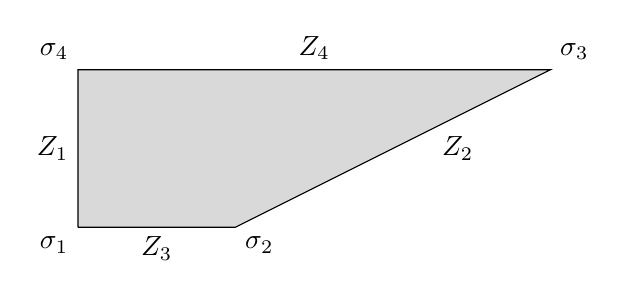
\begin{tikzpicture}
 \draw[fill=gray!30] (0,0)node[below left]{$\sigma_1$} --node[below]{$Z_3$} (2,0)node[below right]{$\sigma_2$} --node[right=.5cm]{$Z_2$} (6,2)node[above right]{$\sigma_3$} --node[above]{$Z_4$} (0,2)node[above left]{$\sigma_4$} --node[left]{$Z_1$} (0,0);
 \end{tikzpicture}
\end{center}
The cohomology ring is given by:
\[
 H^*(\mathbb F_2,\ZZ)\simeq\ZZ[Z_1,\ldots,Z_4]/\langle Z_1-Z_2,Z_4-Z_3-2Z_2, Z_1Z_2,Z_3Z_4\rangle
\]
We work out the following weights for the $\Gm^4$-action:

When thinking of them as curve classes, we'll write $F=[Z_1], D_0=[Z_4], D_\infty=[Z_3]$.

\begin{center}
 \begin{tabular}{||c|c||c|c||}
  \hline\hline
  $\lambda^{\sigma_1}_{\sigma_2}=-\lambda^{\sigma_2}_{\sigma_1}$ & $\lambda_1-\lambda_2$ & $\lambda^{\sigma_3}_{\sigma_4}=-\lambda^{\sigma_4}_{\sigma_3}$ & $\lambda_2-\lambda_1$ \\
  \hline
  $\lambda^{\sigma_2}_{\sigma_3}=-\lambda^{\sigma_3}_{\sigma_2}$ & $2\lambda_1+\lambda_3-\lambda_4$ & $\lambda^{\sigma_4}_{\sigma_1}=-\lambda^{\sigma_1}_{\sigma_4}$ & $\lambda_4-2\lambda_2-\lambda_3$ \\
  \hline\hline
 \end{tabular}
\end{center}

We are going to consider the space $\Q{0}{3}{\mathbb F_2}{D_\infty+F}$ (and the analogous stable maps space) with insertions $\xi_1=Z_3,\xi_2=Z_4,\xi_3=Z_1Z_4$.

The relevant graphs in the stable maps case are:
\begin{center}
 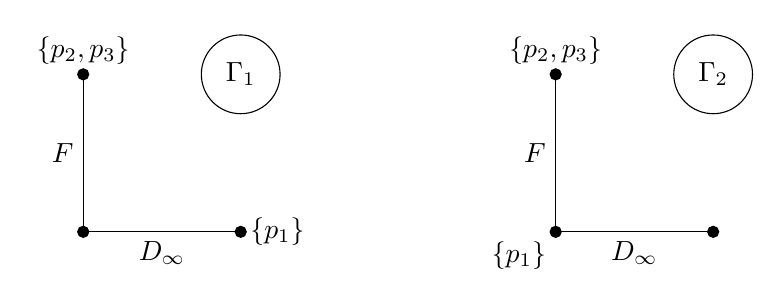
\begin{tikzpicture}[radius=2pt]
  \draw[fill=black] (0,2) circle node[above]{$\{p_2,p_3\}$};
  \draw[fill=black] (0,0) circle;
  \draw[fill=black] (2,0) circle node[right]{$\{p_1\}$};
  \draw (0,2) --node[left]{$F$} (0,0) -- node[below]{$D_\infty$} (2,0);
  \draw (2,2) circle (.5cm) node{$\Gamma_1$};
  %
  \draw[fill=black] (6,2) circle node[above]{$\{p_2,p_3\}$};
  \draw[fill=black] (6,0) circle node[below left]{$\{p_1\}$};
  \draw[fill=black] (8,0) circle;
  \draw (6,2) --node[left]{$F$} (6,0) -- node[below]{$D_\infty$} (8,0);
  \draw (8,2) circle (.5cm) node{$\Gamma_2$};
 \end{tikzpicture}
\end{center}
In the case of quasimaps $\Gamma_2$ is unstable instead the following graph must be taken into account:
\begin{center}
 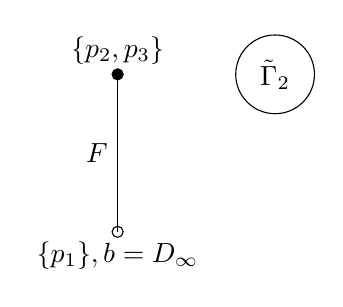
\begin{tikzpicture}[radius=2pt]
  \draw[fill=black] (0,2) circle node[above]{$\{p_2,p_3\}$};
  \draw[fill=white] (0,0) circle node[below]{$\{p_1\},b=D_\infty$};
  \draw (0,2) --node[left]{$F$} (0,0);
  \draw (2,2) circle (.5cm) node{$\tilde\Gamma_2$};
 \end{tikzpicture}
\end{center}
The white circle is supposed to indicate that there is a full basepoint component at that vertex.


\section{Quasimap cohomology and the Batyrev ring}

recap on results from CFK-wallcrossing --> quasimap cohomology in the semi-positive case (issue: the unit, associativity, etc.)

quasimap = quantum in the Fano case

quasimap = Batyrev in the semi-positive non-Fano case via quantum differential equations


%\appendix

\bibliographystyle{alpha}
\bibliography{relqm}

\bigskip\bigskip

%\noindent Luca Battistella\\
%Department of Mathematics, Imperial College London \\
%\texttt{l.battistella14@imperial.ac.uk}\\

%\noindent Navid Nabijou \\
%Department of Mathematics, Imperial College London \\
%\texttt{navid.nabijou09@imperial.ac.uk}



\end{document}